\documentclass[11pt,letterpaper]{article}
\usepackage[margin=1.9cm]{geometry}
\usepackage{fontspec}
\usepackage[provide=*,spanish]{babel}
\usepackage{xcolor}
\usepackage{graphicx}
\usepackage{booktabs}
\usepackage{tabularx}
\usepackage{array}
\usepackage{amsmath,amssymb}
\usepackage{float}
\usepackage{hyperref}

\IfFontExistsTF{DejaVu Sans}{\setmainfont{DejaVu Sans}}{\setmainfont{Arial}}
\IfFontExistsTF{DejaVu Sans Mono}{\setmonofont{DejaVu Sans Mono}}{\setmonofont{Courier New}}

\definecolor{ElectricBlue}{HTML}{0066FF}
\definecolor{NeonCyan}{HTML}{00FFFF}
\definecolor{DarkGray}{HTML}{1E1E1E}
\definecolor{SoftBlue}{HTML}{EEF6FF}
\definecolor{MidBlue}{HTML}{BFD7FF}
\definecolor{Success}{HTML}{087F5B}
\definecolor{Warning}{HTML}{C2410C}

\hypersetup{colorlinks=true,linkcolor=ElectricBlue,urlcolor=ElectricBlue,citecolor=Success,
  pdftitle={Laboratorio 6 - Calculadora Neuronal},pdfauthor={Pablo Daniel Barillas Moreno}}
\pagestyle{plain}
\setlength{\parindent}{0pt}
\setlength{\parskip}{6pt}
\renewcommand{\arraystretch}{1.25}

\newcommand{\metric}[2]{%
  \fcolorbox{MidBlue}{SoftBlue}{\begin{minipage}[c][1.45cm][c]{0.27\textwidth}
  \centering\textcolor{ElectricBlue}{\Large\bfseries #1}\\[-1pt]\small #2
  \end{minipage}}}
\newcommand{\callout}[2]{%
  \begin{center}\fcolorbox{ElectricBlue}{SoftBlue}{\begin{minipage}{0.92\textwidth}
  \textcolor{ElectricBlue}{\bfseries #1}\quad #2
  \end{minipage}}\end{center}}
\newcommand{\code}[1]{\texttt{#1}}

\begin{document}

\begin{titlepage}
\pagecolor{DarkGray}\color{white}
\vspace*{1.5cm}
{\small\bfseries\color{NeonCyan} UNIVERSIDAD DEL VALLE · DEEP LEARNING 2026 · SECCIÓN 30\par}
\vspace{1.2cm}
{\fontsize{36}{42}\selectfont\bfseries Calculadora\\Neuronal\par}
\vspace{.45cm}
{\Large Seq2seq con atención aditiva de Bahdanau\par}
\vspace{1cm}
\colorbox{ElectricBlue}{\parbox{0.87\textwidth}{\color{white}\large
Una evaluación reproducible de aprendizaje aritmético carácter por carácter, atención dinámica,
generalización por longitud y límites adversariales.}}
\vfill
\begin{tabularx}{\textwidth}{@{}lX@{}}
\textcolor{NeonCyan}{\bfseries Estudiante} & Pablo Daniel Barillas Moreno \\
\textcolor{NeonCyan}{\bfseries Carné} & 22193 \\
\textcolor{NeonCyan}{\bfseries Modalidad} & Individual \\
\textcolor{NeonCyan}{\bfseries Fecha} & 2 de octubre de 2026 \\
\textcolor{NeonCyan}{\bfseries Repositorio} & \href{https://github.com/DanielBarillasM/Laboratorio-6_Daniel-Barillas_22193_DLYSI_Sec-30}{GitHub · Laboratorio 6}
\end{tabularx}
\vspace{1cm}
{\color{MidBlue}\rule{\textwidth}{1pt}}\\[5pt]
{\small Paleta Tech Innovation · informe generado desde resultados reales del notebook}
\end{titlepage}
\nopagecolor\color{DarkGray}

\tableofcontents
\clearpage

\section{Resumen ejecutivo}

Este laboratorio estudia si una red neuronal recurrente puede aprender a sumar y restar observando pares
de texto, sin recibir reglas aritméticas explícitas. La entrada es una expresión como
\code{4821+3976}; la salida se genera carácter por carácter. Se implementó una arquitectura encoder--decoder
con GRU bidireccional, atención aditiva y un decoder autoregresivo. El análisis compara tres modelos:
baseline con atención, baseline con contexto fijo y variante de torneo con la salida invertida.

\begin{center}
\metric{97.20\%}{validación · torneo}\hfill
\metric{95.00\%}{cuatro cifras · torneo}\hfill
\metric{186,767}{parámetros}
\end{center}

La modificación controlada \code{invertir\_salida=True} mejoró 13.50 puntos porcentuales la validación
global y 24.67 puntos la exactitud de cuatro cifras respecto del baseline con atención. No incrementó el
número de parámetros, ejemplos o épocas. Sin embargo, el modelo obtuvo 0\% en cinco y seis cifras y falló
en cinco casos válidos cuidadosamente buscados. La conclusión es doble: la inductiva escogida facilita el
acarreo dentro de la distribución, pero no produce un algoritmo simbólico universal.

\callout{Estado de entrega.}{El notebook fue ejecutado desde un kernel reiniciado hasta la celda de
Entrega. El formulario confirmó el registro y la huella del modelo de torneo se mantuvo en
\code{94e198ec75ec}. La clave del torneo sigue en \code{None} porque corresponde al Laboratorio 7.}

\section{Problema, objetivos y alcance}

\subsection{Pregunta central}

La tarea exige transformar una secuencia de caracteres de longitud variable en otra secuencia. Aunque las
sumas y restas siguen reglas deterministas, una red entrenada por gradiente solo observa ejemplos. Para
resolver correctamente debe representar operandos, operación, posición decimal, acarreos o préstamos y
la condición de finalización de la salida.

Los objetivos concretos fueron:
\begin{itemize}
  \item implementar la atención aditiva de Bahdanau y un paso del decoder;
  \item comparar atención dinámica contra un único contexto fijo;
  \item medir exactitud exacta por cantidad de cifras;
  \item formular y probar una mejora de torneo con una o dos perillas;
  \item localizar cinco contraejemplos dentro del rango permitido;
  \item conservar pesos, huellas, métricas, figuras y notebook ejecutado.
\end{itemize}

\subsection{Restricciones de la guía}

El entrenamiento usa CPU, PyTorch, Matplotlib y biblioteca estándar. No se utiliza NumPy ni la capa
\linebreak\code{nn.MultiheadAttention}. Los operandos de entrenamiento no exceden cuatro cifras, la arquitectura no
se modifica en el bloque de torneo y el modelo debe permanecer por debajo de 750,000 parámetros. Las
celdas oficiales de verificación se preservaron sin cambios.

\begin{table}[H]\centering
\caption{Matriz de requisitos principales.}
\begin{tabularx}{\textwidth}{>{\bfseries}p{.25\textwidth}X>{\raggedleft\arraybackslash}p{.18\textwidth}}
\toprule Requisito & Evidencia & Estado \\
\midrule
Atención aditiva & Formas, normalización y máscara verificadas & Cumple \\
Paso del decoder & Logits, estado y pesos verificados & Cumple \\
Exactitud base $\geq 0.60$ & Exactitud 0.837 & Cumple \\
Máximo 750,000 parámetros & 186,767 parámetros & Cumple \\
Cinco trampas válidas & Cinco fallos reproducidos & Cumple \\
Registro externo & Mensaje oficial de confirmación visible & Cumple \\
\bottomrule
\end{tabularx}
\end{table}

\clearpage
\section{Fundamento teórico}

\subsection{Del vector fijo al contexto dinámico}

En un encoder--decoder clásico, toda la entrada se resume en un vector fijo. Bahdanau, Cho y Bengio
identifican este mecanismo como un cuello de botella: a medida que crece la secuencia, el resumen debe
preservar demasiados detalles. La atención sustituye esa única decisión global por un contexto específico
para cada paso de salida \cite{bahdanau2014}.

Sea $s$ el estado actual del decoder y $h_j$ el estado del encoder asociado con el carácter $j$:
\begin{align}
e_j &= v^\top \tanh(W_qs+W_kh_j),\\
\alpha_j &= \frac{\exp(e_j)}{\sum_k\exp(e_k)},\\
c &= \sum_j\alpha_jh_j.
\end{align}
Los puntajes de posiciones de relleno se sustituyen por $-\infty$ antes del \emph{softmax}; por tanto,
su peso es exactamente cero. El contexto $c$ permite al decoder consultar distintas regiones de la
expresión mientras genera cada dígito.

\subsection{Orden de secuencia y distancia de dependencias}

Sutskever, Vinyals y Le mostraron que invertir la fuente podía reducir la distancia mínima entre elementos
relacionados de entrada y salida y facilitar la optimización \cite{sutskever2014}. La aritmética decimal
sugiere una adaptación más específica: una persona suma desde las unidades y propaga el acarreo hacia la
izquierda. Si el decoder escribe la respuesta en orden convencional, debe predecir primero el dígito más
significativo, que puede depender de un acarreo originado varias columnas a la derecha.

La hipótesis previa al entrenamiento fue entonces: invertir únicamente la salida hará que el decoder genere
unidades primero y almacene el acarreo en su estado recurrente. La entrada se conservó intacta para aislar
una sola modificación.

\section{Datos sintéticos y capacidad de memorización}

Cada ejemplo se genera al azar; los operandos tienen de una a cuatro cifras, la operación es suma o resta
y las restas nunca son negativas. El vocabulario tiene 15 símbolos: diez dígitos, dos operadores y tres
tokens especiales.

Para dos operandos de exactamente cuatro cifras existen $9,000^2=81,000,000$ sumas ordenadas. En restas
no negativas, los pares con $a\geq b$ son
\[
\frac{9,000(9,000+1)}{2}=40,504,500.
\]
El total asciende a 121,504,500 expresiones, frente a solo 40,000 ejemplos de entrenamiento. La muestra
representa menos de 0.033\% de ese subconjunto; el modelo no puede memorizar exhaustivamente el espacio y
debe generalizar regularidades.

\begin{figure}[H]\centering
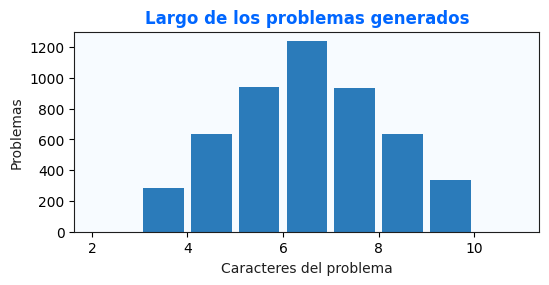
\includegraphics[width=.82\textwidth]{../artifacts/figuras/01_distribucion_longitudes.png}
\caption{Distribución de longitudes en la validación reproducible.}
\end{figure}

\clearpage
\section{Arquitectura e implementación}

\subsection{Encoder}

El encoder convierte caracteres en embeddings y usa una GRU bidireccional. Se emplea la función
\linebreak\code{pack\_padded\_sequence} para impedir que la recurrencia procese el padding. Las dos direcciones se
concatenan tanto en las salidas posicionales como en el resumen global; un puente lineal produce el estado
inicial del decoder.

\subsection{Atención}

La implementación usa proyecciones lineales sin sesgo para consulta y claves, activación hiperbólica,
proyección escalar, máscara y \code{torch.bmm} para la suma ponderada. La verificación oficial comprueba:
\begin{itemize}
  \item pesos de forma $(B,T)$ y contexto de forma $(B,d_{enc})$;
  \item suma de pesos igual a uno por ejemplo;
  \item peso exactamente cero en posiciones \code{<PAD>}.
\end{itemize}

\subsection{Decoder}

En cada paso, el token previo se embebe; la atención calcula un contexto desde el estado actual; una
\code{GRUCell} recibe la concatenación $[embedding, contexto]$; y la capa final recibe
$[nuevo\_estado, contexto]$. Durante el entrenamiento se usa \emph{teacher forcing}; durante la inferencia,
el token predicho realimenta el paso siguiente.

\subsection{Complejidad}

Los tres modelos contienen 186,767 parámetros. El baseline sin atención conserva los módulos de atención
aunque no los consulta, por lo que el conteo coincide; esto mantiene la clase y el formato de checkpoint
uniformes. La capacidad utilizada equivale a 24.9\% del máximo permitido.

\section{Diseño experimental}

\begin{table}[H]\centering
\caption{Configuración compartida y variable experimental.}
\begin{tabular}{lccc}
\toprule & Con atención & Sin atención & Torneo \\
\midrule
Ejemplos & 40,000 & 40,000 & 40,000 \\
Épocas & 15 & 15 & 15 \\
Dimensión embedding & 32 & 32 & 32 \\
Dimensión oculta & 64 & 64 & 64 \\
Tasa de aprendizaje & 0.003 & 0.003 & 0.003 \\
Semilla & 2026 & 2026 & 2026 \\
Atención & Sí & No & Sí \\
Salida invertida & No & No & Sí \\
\bottomrule
\end{tabular}
\end{table}

La exactitud exige coincidencia completa de la cadena; un solo dígito incorrecto vuelve incorrecto todo el
ejemplo. La validación global usa 2,000 problemas. La evaluación por longitud usa 300 problemas para cada
nivel de una a seis cifras, donde cinco y seis son estrictamente fuera del rango de entrenamiento.

La comparación del torneo mantiene semilla, muestra, épocas, optimizador y capacidad. Esto fortalece la
atribución causal a la inversión de salida, aunque una sola semilla no permite estimar variabilidad entre
entrenamientos.

\clearpage
\section{Resultados}

\subsection{Aprendizaje durante 15 épocas}

\begin{figure}[H]\centering
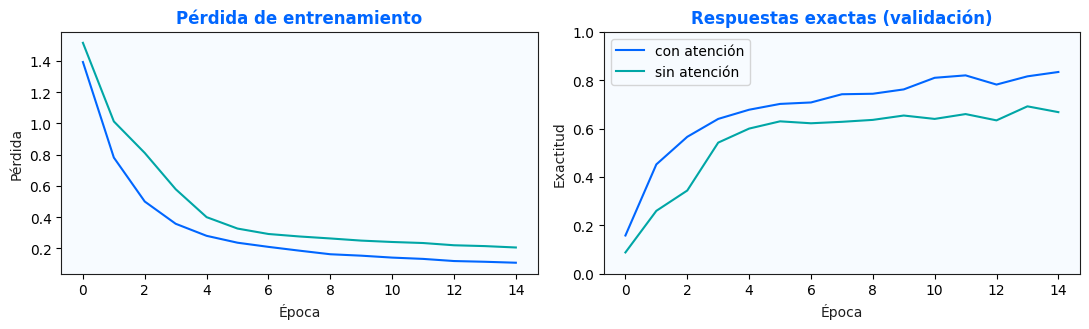
\includegraphics[width=.94\textwidth]{../artifacts/figuras/02_curvas_entrenamiento.png}
\caption{Pérdida y exactitud de validación por época para ambos baselines.}
\end{figure}

El baseline con atención finalizó con 83.70\% de exactitud global, 16.45 puntos por encima del modelo con
contexto fijo. Las curvas no son estrictamente monótonas: la exactitud exacta puede fluctuar aunque la
pérdida por token disminuya, porque basta un token erróneo para invalidar una respuesta completa.

\begin{table}[H]\centering
\caption{Resultados globales, capacidad e identidad de pesos.}
\begin{tabular}{lrrl}
\toprule Modelo & Validación & Parámetros & Huella \\
\midrule
Base con atención & 83.70\% & 186,767 & \code{7dd56f9acf5d} \\
Base sin atención & 67.25\% & 186,767 & \code{11a6346d696d} \\
Torneo, salida invertida & \textbf{97.20\%} & 186,767 & \code{94e198ec75ec} \\
\bottomrule
\end{tabular}
\end{table}

\subsection{Efecto de la atención por longitud}

\begin{figure}[H]\centering
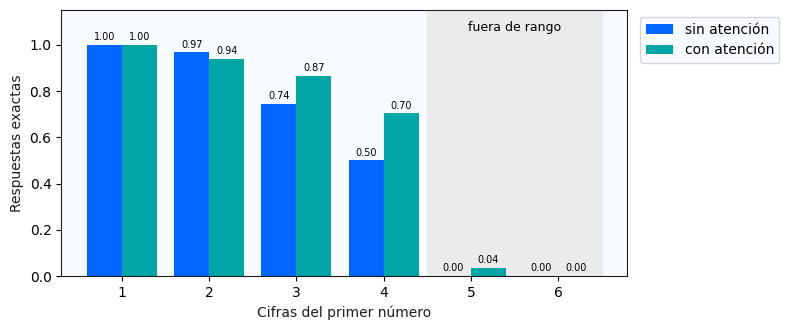
\includegraphics[width=.88\textwidth]{../artifacts/figuras/03_exactitud_por_cifras_baselines.png}
\caption{Exactitud del baseline con y sin atención por cantidad de cifras.}
\end{figure}

Con un dígito no hay diferencia; con dos, el modelo fijo es ligeramente superior. En tres y cuatro cifras,
la atención obtiene 86.67\% y 70.33\%, frente a 74.33\% y 50.00\%. Esto apoya la explicación del cuello
de botella: la selección dinámica se vuelve valiosa conforme crece la secuencia.

\clearpage
\subsection{Prueba de la hipótesis del torneo}

\begin{figure}[H]\centering
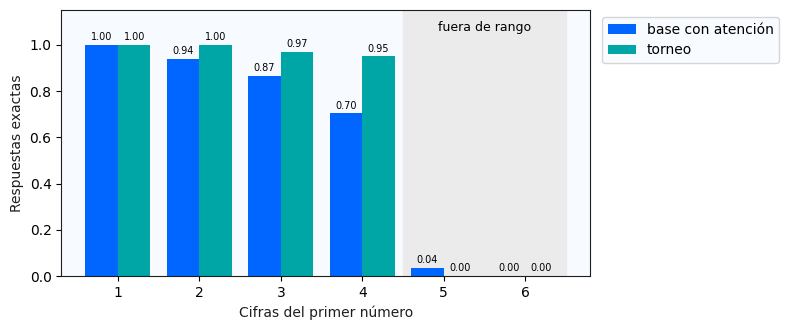
\includegraphics[width=.88\textwidth]{../artifacts/figuras/05_exactitud_base_vs_torneo.png}
\caption{Comparación controlada entre el baseline con atención y la salida invertida.}
\end{figure}

\begin{table}[H]\centering
\caption{Exactitud exacta por longitud.}
\begin{tabular}{rrrr}
\toprule Cifras & Con atención & Sin atención & Torneo \\
\midrule
1 & 100.00\% & 100.00\% & 100.00\% \\
2 & 94.00\% & 96.67\% & 100.00\% \\
3 & 86.67\% & 74.33\% & 97.00\% \\
4 & 70.33\% & 50.00\% & \textbf{95.00\%} \\
5, fuera de rango & 3.67\% & 0.00\% & 0.00\% \\
6, fuera de rango & 0.00\% & 0.00\% & 0.00\% \\
\bottomrule
\end{tabular}
\end{table}

La hipótesis se cumple: invertir la salida mejora la métrica objetivo y no sacrifica la validación global.
La mejora es compatible con una reducción de la dificultad temporal del acarreo. No obstante, el cero por
ciento fuera de rango muestra que la intervención mejora interpolación y no extrapolación de longitud.

\section{Interpretación de la atención}

\begin{figure}[H]\centering
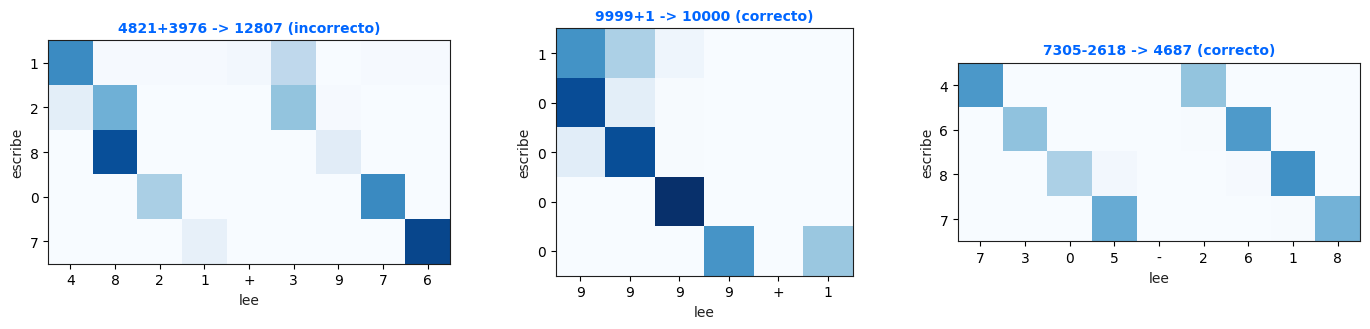
\includegraphics[width=.98\textwidth]{../artifacts/mapas_atencion/04_atencion_baseline.png}
\caption{Mapas del baseline con atención para tres expresiones.}
\end{figure}

En el baseline, el peso cambia entre pasos de salida y se concentra en regiones diferentes de los
operandos. En \code{4821+3976} se observan alineaciones posicionales, pero no una diagonal perfecta que
equivalga a la suma por columnas. El decoder convencional escribe primero la izquierda, mientras el
acarreo surge a la derecha, lo que obliga al estado a anticipar dependencias de largo alcance.

\begin{figure}[H]\centering
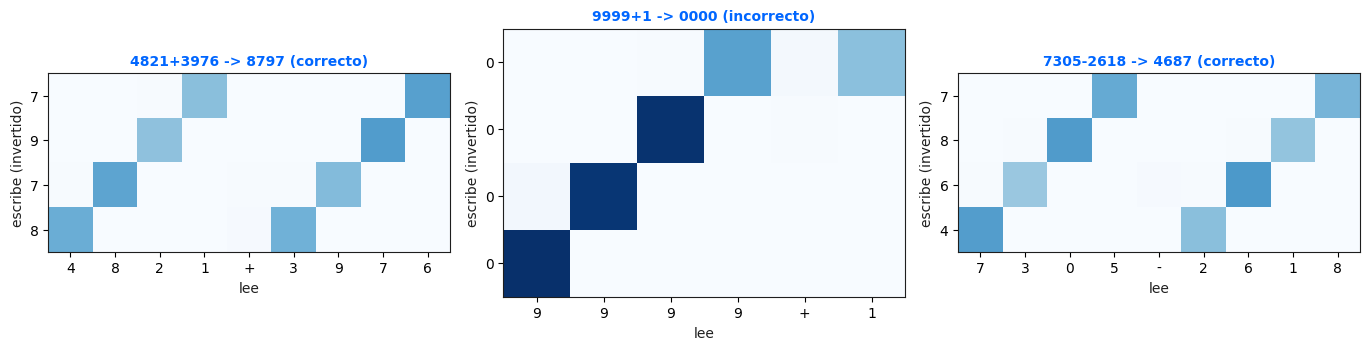
\includegraphics[width=.98\textwidth]{../artifacts/mapas_atencion/06_atencion_torneo.png}
\caption{Mapas del modelo de torneo; la salida se genera internamente en orden invertido.}
\end{figure}

En el modelo de torneo las filas deben leerse en orden de generación interno: unidades antes que cifras de
mayor valor. Esta representación temporal es más congruente con el acarreo. Sin embargo, un mapa de
atención muestra distribución de pesos, no una prueba causal de que cada celda implemente una operación
simbólica.

\clearpage
\section{Análisis adversarial}

Se exploraron primero familias difíciles ---acarreos completos, préstamos a través de ceros, resultados
cortos y cambios de longitud--- y luego una búsqueda determinista de hasta 15,000 expresiones válidas.
Los primeros cinco fallos distintos fueron:

\begin{table}[H]\centering
\caption{Casos que rompen el modelo final dentro del rango permitido.}
\begin{tabularx}{\textwidth}{lrrX}
\toprule Problema & Predicción & Correcta & Interpretación \\
\midrule
\code{9999+1} & \code{0000} & \code{10000} & Acarreo global y nueva cifra \\
\code{9998+2} & \code{0000} & \code{10000} & Acarreo desde unidades \\
\code{9999+9999} & \code{18998} & \code{19998} & Acarreos simultáneos \\
\code{1000-999} & \code{11} & \code{1} & Préstamo y longitud de salida \\
\code{4000-3999} & \code{001} & \code{1} & Préstamos y ceros iniciales \\
\bottomrule
\end{tabularx}
\end{table}

\begin{figure}[H]\centering
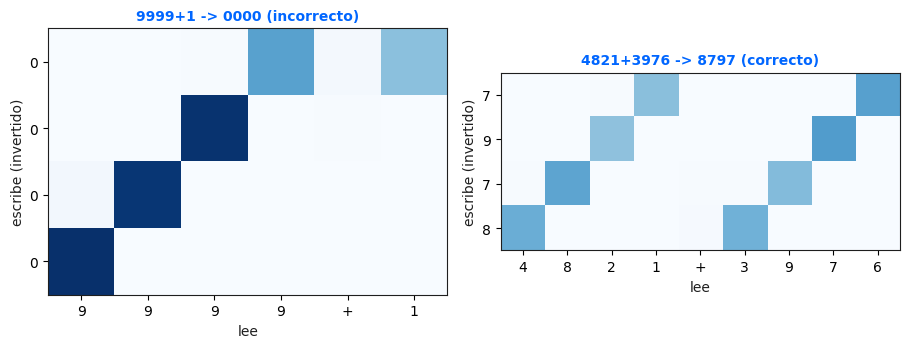
\includegraphics[width=.88\textwidth]{../artifacts/mapas_atencion/07_trampa_vs_control.png}
\caption{Comparación entre \code{9999+1} y el caso de control \code{4821+3976}.}
\end{figure}

El caso \code{9999+1} exige producir cinco dígitos a partir de operandos de cuatro y propagar un acarreo por
todas las columnas. El modelo produce \code{0000}: capta una parte del patrón local, pero omite la nueva
cifra significativa. La evidencia respalda que aprendió a imitar muchas operaciones dentro de la
distribución, no una regla universal. Un único contraejemplo basta para refutar universalidad; aquí se
presentan cinco.

\section{Reproducibilidad y trazabilidad}

El repositorio conserva el machote original, el notebook final con salidas, tres checkpoints, métricas
JSON, figuras exportadas y documentación por tarea. Los scripts reconstruyen el notebook, ejecutan dos
etapas sin enviar el formulario, exportan figuras y verifican la entrega.

\begin{verbatim}
python scripts/build_notebook.py
python scripts/execute_notebook.py --stage discover
python scripts/build_notebook.py
python scripts/execute_notebook.py --stage final
python scripts/exportar_figuras.py
python scripts/verificar_entrega.py
\end{verbatim}

El notebook contiene 15 celdas de código ejecutadas con conteos consecutivos y sin errores hasta la
entrega. La salida del formulario confirma el envío y repite la huella \code{94e198ec75ec}. La única celda
sin ejecutar es la del torneo; \code{CLAVE=None} se mantiene hasta que el profesor revele la clave del
Laboratorio 7.

La metodología de producción y revisión de visualizaciones siguió principios de evidencia, legibilidad y
reproducción asistida descritos por Kassis et al. \cite{kassis2026}; esa referencia documenta el proceso,
no sustituye las fuentes académicas de atención y seq2seq.

\section{Conclusiones}

\begin{enumerate}
  \item La atención aporta una ventaja clara cuando crece la longitud dentro de la distribución: 20.33
  puntos en cuatro cifras respecto del contexto fijo.
  \item Invertir la salida es una intervención pequeña y eficaz: lleva la exactitud de cuatro cifras a
  95.00\% y la validación global a 97.20\% sin sumar parámetros.
  \item La visualización de atención ayuda a inspeccionar alineaciones, pero no demuestra razonamiento
  simbólico ni causalidad interna.
  \item La generalización de longitud es deficiente: el modelo de torneo cae a 0\% con cinco y seis cifras.
  \item Los fallos en acarreos globales y préstamos entre ceros prueban que una métrica promedio alta debe
  complementarse con evaluación adversarial.
\end{enumerate}

Como trabajo futuro, se recomienda repetir el experimento con múltiples semillas, separar conjuntos por
familias de acarreo y préstamo, evaluar exactitud por token además de cadena completa y estudiar currículos
que aumenten progresivamente la longitud. Cualquier cambio para el torneo deberá respetar la arquitectura,
el máximo de cuatro cifras durante entrenamiento y la huella ya registrada.

\addcontentsline{toc}{section}{Referencias}
\begin{thebibliography}{9}
\bibitem{bahdanau2014}
D. Bahdanau, K. Cho y Y. Bengio.
\emph{Neural Machine Translation by Jointly Learning to Align and Translate}.
arXiv:1409.0473, 2014. \url{https://arxiv.org/abs/1409.0473}

\bibitem{sutskever2014}
I. Sutskever, O. Vinyals y Q. V. Le.
\emph{Sequence to Sequence Learning with Neural Networks}.
arXiv:1409.3215, 2014. \url{https://arxiv.org/abs/1409.3215}

\bibitem{kassis2026}
T. Kassis, V. Agarwal, Y. He, D. Patel y A. M. Brueckner.
\emph{Scientific Agent Skills: A Library of Procedural Knowledge for Research Agents}.
arXiv:2609.00065, 2026. \url{https://doi.org/10.48550/arXiv.2609.00065}
\end{thebibliography}

\section*{Declaración de apoyo con IA}

Se utilizó IA como apoyo de ingeniería para estructuración, revisión, automatización y presentación. Las
afirmaciones académicas se sustentan en las fuentes citadas; la IA no se considera una fuente. Todas las
métricas, predicciones, huellas y figuras reportadas provienen de la ejecución reproducible incluida.

\end{document}
